\documentclass{article}
\usepackage{dennis}

\usepackage{float}

\title{Integration}
\author{Dennis Chen and Dylan Yu}
\date{2021}

\begin{document}
\maketitle

Just like in differentiation, where we want to reconcile two different definitions -- the approximation-based definition and the repeated differentiation-based definition -- we want to take the two different definitions of the integral and understand why they're really the same: the area under a curve definition and the antiderivative definition. We unify the two definitions with the \db{Fundamental Theorem of Calculus}.

\section{The Integral}

Because integration can be somewhat hard to grasp at the beginning, we spend a lot of time bashing you over the head with the ``area under a curve'' and antiderivative concepts. If you find yourself going ``I understand all of this, and this is going very slowly,'' feel free to skim/skip the section \db{until you get to the Fundamental Theorem of Calculus}.

\subsection{Area Under a Curve and Some Exposition}

We crudely define the integral as the area under a curve.\footnote{If you want a non-terrible definition, you'll have to wait until real analysis.}

The purpose of the antiderivative is to answer the question: if $F'(x)=f(x)$, and we are given $f$, what is $F$? You'll soon see that a function has infinitely many antiderivatives, and all differ only by a constant. Furthermore, just like the derivative of $f$ may not exist, the antiderivative can also be non-existent.

\begin{defi}[Integral]
For a function $f$ that is continuous over $[a,b],$ we define the \db{integral} $\int\limits_{a}^{b}f(x)dx$ as the area under $f$ in the range $[a,b].$

If $f$ goes below the $y$ axis, then the area counts as negative.
\end{defi}

\begin{defi}[Indefinite Integral]
Let $f(x)$ be a function that has an antiderivative $F(x)$. The \db{indefinite integral} of $f(x)$ is denoted by and equal to
$$\int f(x)\,dx = F(x)+C,$$
where $C$ is a constant.
\end{defi}
\begin{defi}[Definite Integral]
Let $f(x)$ be a function that has an antiderivative $F(x)$. The \db{definite integral} of $f(x)$ from $x=a$ to $x=b$ is denoted by and equal to
$$\int_a^b f(x)\, dx=F(b)-F(a)=\Eval{F(x)}{a}{b}.$$
\end{defi}

% physics applications

We use the area under a curve definition to extract a couple of (probably obvious) facts about integrals.

\begin{theo}[Integral Properties]
For a function $f$ that is continuous over $[a,b],$ where all variables in the integrals are assumed to be in the range $[a,b],$ the following are true:
\begin{itemize}
\item Joining integrals: $\int\limits_{a}^{c}f(x)dx+\int\limits_{c}^{b}f(x)dx=\int\limits_a^b f(x)dx.$\footnote{Actually, provided that the function is continuous over the right interval, $c$ does not have to be between $a$ and $b$.}

\item Linearity of integrals: $\int\limits_{a}^{b}(pf(x)+qg(x))d(x)=p\int\limits_{a}^{b}f(x)dx+q\int\limits_{a}^{b}g(x)dx.$
\end{itemize}
\end{theo}

This limited understanding of integration is enough to do the most basic of mechanics problems, so we do a couple of them as examples.

\begin{exam}
A car is accelerating at $1 m/s^2$ (meter per second squared). If the car starts at a speed of $0$ meters, find the distance the car has traveled after it reaches a speed of $60 m/s.$
\end{exam}

\begin{sol}
Note that the condition is just code for ``how far does the car travel after $60$ seconds?'' So we just need to integrate $\int\limits_{0}^{60}xdx.$ Note that this is an isosceles right triangle with side length $60,$ so the area is just $\frac{60^2}{2}=1800.$ Thus the car has traveled $1800$ meters.
\begin{center}
\begin{tikzpicture}[scale=0.06]
\filldraw[color=thmblue] (0,0)--(60,0)--(60,60)--cycle;
\draw (60,0)--(0,0)--(0,60);
\draw[color=dennispurple] (0,0)--(60,60);
\node at (40,40) [anchor=south east]{$y=x$};
\node at (0,0) [anchor = north east]{$0$};
\node at (60,0) [anchor = north]{$60$};
\node at (0,60) [anchor=east]{$60$};
\end{tikzpicture}
\end{center}
\end{sol}

\begin{exam}[Negative Area]
A car is going in reverse at $-10 m/s$ and accelerating at $1 m/s^2.$ How far is the car from its original position after $70$ seconds?
\end{exam}

\begin{sol}
Note that the red area below the $y$ axis represents the car going backwards, so we subtract it from the overall integral. Thus $\int_{0}^{70}xdx=\frac{60^2}{2}-\frac{10^2}{2}=1750,$ and the car is $1750$ meters away from its original position.
\begin{center}
\begin{tikzpicture}[scale=0.06]
\filldraw[color=thmblue] (10,0)--(70,0)--(70,60)--cycle;
\filldraw[color=thmred] (0,-10)--(0,0)--(10,0)--cycle;
\draw (70,0)--(0,0)--(0,60);
\draw (0,-10)--(0,0);
\draw[color=dennispurple] (70,60)--(0,-10);
\node at (50,40) [anchor=south east]{$y=x-10$};
\node at (0,0) [anchor = east]{$0$};
\node at (0,-10) [anchor = north east] {$-10$};
\node at (70,0) [anchor = north]{$70$};
\node at (0,60) [anchor=east]{$60$};
\node at (11,0) [anchor = north] {$10$};
\end{tikzpicture}
\end{center}
\end{sol}

If the concept of negative area is confusing, just use the linearity of integrals to shift the function up by a constant, and adjust for it by subtracting the area of a rectangle at the end.\footnote{After you think of this, the concept is probably going to be less confusing anyways...}

There are dozens of these types of practice problems in any standard high-school calculus textbook, particularly because it is very easy to draw lines on a graph and ask for the area under said lines. If you want practice on these problems, you can probably get away with doing the same thing yourself and finding the area -- this is just simple geometry.\footnote{I do not think spamming these sorts of exercises are the right thing to do anyway, because you either spend a lot of time missing the point or you've already gotten the point anyways. The only real consideration you have to make is towards negative areas, and shifting the function by a constant explains the motivation behind this very well.}

\subsection{Antiderivatives}

Because the derivative is a function, it has an inverse. We examine the inverse, known as the antiderivative.

\begin{defi}[Antiderivative]
The antiderivative of a function $f(x)$ is the function $F$ that satisfies $F'(x)=f(x).$
\end{defi}

The antiderivative is not unique, and the possible antiderivatives differ by a constant.

\begin{theo}[Constant perturbance]
If $F'(x)=f(x)$ and $g(x)=F(x)+C$ for any constant $C,$ then $g'(x)=F(x).$
\end{theo}

\begin{pro}
We use the fact that derivatives are additive. Note that
\[g'(x)=(F(x)+C)'=F'(x),\]
as desired.
\end{pro}

Now how do we go about finding the antiderivative? The Power Rule makes it very easy to find the antiderivatives for polynomials:

\begin{exer}[Antiderivative with Power Rule]
Prove that the antiderivative of $x^n$ is $nx^{n+1}+C$ for all $x\neq -1.$
\end{exer}

\begin{exer}[Followup to Power Rule]
Why is $x=-1$ the exception, and what is the antiderivative of $\frac{1}{x}?$
\end{exer}

In theory, we could take the Maclaurin Series of any function and then find the antiderivative of each term. But this is often more trouble than it's worth, so here's a list of antiderivatives you should know.

\begin{theo}[Common Antiderivatives] % fill in trig, power rule, 1/x, arc(sin/cos/tan), e^{f(x)}
We might mention a few of these later, so take them for granted for now:
\begin{itemize}
    \item $\int x^n\,dx=\frac{1}{n+1}x^{n+1}+C,n\neq -1$
    \item $\int \sin(x)\, dx=-\cos(x)+C$
    \item $\int \cos(x)\,dx=\sin(x)+C$
    \item $\int\sec^2x\,dx=\tan(x)+C$
    \item $\int e^x\,dx=e^x+C$
    \item $\int\sinh(x)\,dx=\cosh(x)+C$
    \item $\int\cosh(x)\,dx=\sinh(x)+C$
    \item $\int\frac{1}{x}\,dx=\ln|x|+C$
    \item $\int\frac{1}{1-x^2}\,dx=\arcsin(x)+C$
    \item $\int\frac{1}{1+x^2}\,dx=\arctan(x)+C$
    \item $\int\frac{1}{x\sqrt{x^2-1}}\,dx=\arcsec(x)+C$
\end{itemize}
\end{theo}

You can easily show most of these by differentiating the right-hand side. Here's a heuristic you should be aware of: \db{whenever you see something of the form $1\pm x^2$ in the denominator of a function}, think trig substitutions.

\begin{exer}[Antiderivative of $e^{f(x)}$]
Show that the antiderivative of $e^{f(x)}$ is $\frac{e^{f(x)}}{f'(x)}.$
\end{exer}

\subsection{Putting it Together}

Now that we've presented the two definitions of the integral, we'll follow up by linking them together with the Fundamental Theorem of Calculus.

\begin{theo}[The Fundamental Theorem of Calculus]\label{theo:fun}
Let $f$ be a continuous function $f$ on $[a,b]$ and let
\[F(x)=\int\limits_{a}^x f(x)dx\]
for all $x\in (a,b),$ where the integral function denotes the area under the curve. Then
\begin{enumerate}
\item For all $x\in (a,b),$ $F'(x)=f(x).$

\item If $f$ and $g$ are continuous on $[a,b]$ and $g'(x)=f(x),$ then $\int\limits_{a}^{b}f(x)dx = g(b)-g(a).$ (In other words, $g(x)=F(x)+C$ for some constant $C.$)
\end{enumerate}
\end{theo}

\begin{pro}
The first part follows from the limit definition of the derivative. I'll explicitly state the key idea: \db{we're adding a rectangle of width $\epsilon$ and height $f(x).$} Note that \[F'(x)=\lim_{\epsilon\to 0}\frac{F(x+\epsilon)-F(x)}{\epsilon}=\lim_{\epsilon\to 0}\frac{\int\limits_{x}^{x+\epsilon}f(x)dx}{\epsilon}=\frac{\epsilon f(x)}{\epsilon}=f(x).\]

The second part follows from the first. Note that if $F'(x)=f(x),$ then by properties of the derivative, the only functions $g$ that satisfy $g'(x)=f(x)$ are of the form $F'(x)+C$ for any constant $C.$ Thus $g(b)-g(a)=F(b)-F(a)=\int\limits_{a}^{b}f(x)dx.$

\begin{center}
\begin{tikzpicture}[scale=1.5]
\draw[->] (-3.1415,0)--(3.1415,0) node[above]{$x$};
\draw[->] (0,-1)--(0,1) node[left]{$y$};
\draw[domain=-3.1415:3.1415] plot(\x,{sin(180/3.1415*\x)});
\filldraw[pattern = north west lines, pattern color = darkblue] (1.04719755,0.866025404) rectangle (1.5, 0);
\node at (1.2735, 0) [below]{$\epsilon$};
\node at (1.04719755, 0.35) [left]{$f(x)$};
\end{tikzpicture}
\end{center}
\end{pro}

The two parts are respectively called the \db{second} and \db{first} fundamental theorems of calculus, respectively.\footnote{I don't know why the theorems are ordered like this either and I think it makes sense to present the second before the first, but if anyone knows why, please shoot me an email at proofprogram@gmail.com or message me on Discord at shootinglucky$\#4186$ so I can replace this footnote with something more useful.}

\subsubsection{Indefinite Integrals}

Now we really connect the idea of integrals and anti-derivatives with the \db{indefinite integral}, which is a representation of an integral as an anti-derivative.

\begin{defi}[Indefinite Integral]
Given $F'(x)=f(x),$ we say that
\[\int f(x)dx=F(x)+C.\]
\end{defi}

In general, we will choose to express the constant term of $F(x)$ as $0,$ since it is neater and $+C$ doesn't really care what the constant term is anyways.

\section{Evaluating the Integral}

Because integrals are really just the reverse of derivatives, it follows that the two fundamental rules of differentiation hold in some for integration: the \db{chain rule} and \db{product rule}. Their counterparts in integration are $u$-substitution (and the use of $u$-substitution is followed by something still called the chain rule) and integration by parts.

\subsection{$u$-substitution}

The chain rule is really just saying that $\frac{d}{dx}=\frac{d}{du}\cdot \frac{du}{dx}.$ When we do a $u$-substitution, what we're really trying to do is \db{get rid of unruly expressions in} $x$ and turn them into managable expressions in terms of $u.$

\begin{theo}[Chain Rule]
If $u$ is a function about $x,$ $g(u)=f(x),$ and $f(x)$ is an integratable function, then $\int f(x) dx = \int \frac{g(u)}{u'}du.$
\end{theo}

This is implied by the chain rule for derivatives.

\begin{exam}
Find $\int 8x(2x^2+1)dx.$
\end{exam}

\begin{sol}
Of course we can just integrate with linearity, but for the sake of this example we will avoid doing that and use $u$-substitution instead.

The ``unruly term'' here is $2x^2+1.$ Note that the derivative of this term is $4x,$ so substituting $u=2x^2+1$ gives
\[\int 8x(2x^2+1)dx=\int \frac{8xu}{u'}du=\int\frac{8xu}{4x}du=\int 2udu=u^2.\]
\end{sol}

If we're dealing with definite integrals, then in our $u$-substitution, \db{we must make sure to change the bounds according to $u$}. Let's reuse the previous example.

\begin{exam}[Changing Bounds]
Find $\int\limits_{-1}^{3} 8x(2x^2+1)dx.$
\end{exam}

\begin{sol}
The bounds have to be expressed in terms of $u$. Since $x=-1$ and $x=3$ are the bounds, the new bounds are $u=2(-1)^2+1=3$ and $u=2(3)^2+1=19.$ Thus the integral is equivalent to
\[\int_{3}^{19}2udu=19^2-3^2=352.\]
\end{sol}

\begin{exer}
This is seemingly suspicious because this implies that $\int\limits_{-a}^{a} 8x(2x^2+1)dx=\int\limits_{2a^2+1}^{2a^2+1}u^2dx=0.$ In other words, $-a$ and $a$ in this case would be indistinguishable as bounds. So why is this correct?
\end{exer} % the original function is odd

\begin{exam}
Find $\int x(2x^3+1)^2.$
\end{exam}

\begin{remark}
One might initially believe that that $u$-sub does not work here: allowing $u=2x^3+1$ gives us
\[\int \frac{1}{6x}u^2 du,\]
and expressing $x$ in terms of $u$ is not even worth the effort.
\end{remark}

\begin{sol}
With a little bit of ingenuity, $u$-substitution will work. If you let $u=x^2$ instead, then you get
\[\int \frac{(2u\sqrt{u}+1)^2}{2}du.\]
At this point, crudely expanding will just work: you get
\[\int \frac{4u^3+4u\sqrt{u}+1}{4}du=\frac{u^4}{4}+\frac{8u^2\sqrt{u}}{5}+u+C=\frac{x^8}{2}+\frac{4x^5}{5}+\frac{x^2}{2}+C.\]
Indeed, there is no good reason to use integration by parts here -- we only presented it as an example that could be verified through other approaches.
\end{sol}

Notice that in these types of integrals, we want to \db{contrive} the $u$-sub into working: Take a value of $u$ that might seem inconvenient at first to force the $x$ to disappear.

Here is a very tricky and non-obvious application of the chain rule: the integral of $\sec x.$

\begin{exam}[sec x]
Find $\int \sec x dx.$
\end{exam}

\begin{sol}
Multiply by $\frac{\sec x+ \tan x}{\sec x + \tan x}$ and make the integral
\[\int \sec x \frac{\sec x + \tan x}{\sec x + \tan x}.\]
Set $u=\sec x + \tan x,$ and then $u'=\sec x \tan x + \sec^2 x.$ Now the integral is equivalent to
\[\int \frac{\frac{\sec^2 x + \sec x \tan x}{\sec x + \tan x}}{u'}du=\int \frac{1}{\sec x + \tan x}du=\int \frac{1}{u} du =\]
\[\ln|u|+C=\ln|\sec x+\tan x|+C.\]
\end{sol}

\begin{exer}[Nearly arctan]
Find $\int \frac{1}{\sqrt{1+x^2}}.$
\end{exer}

\begin{exam}[Reverse $u$-sub]
Find $\int_{-1}^8\sqrt{1+\sqrt{1+x}}\,dx$.
\end{exam}

\begin{sol}
Let $x=u^2-1$ and $dx=2u\,du$. Then we have
$$\int_0^3\sqrt{1+u}\cdot 2u\,du,$$
and we can set $u=t^2-1$ and $du=2t\,dt$ to get
$$\int_1^2  t\cdot2(t^2-1)\cdot 2t\,dt = \Eval{\paren{\frac{4}{5}t^5-\frac{4}{3}t^3}}{1}{2}=\boxed{\frac{232}{15}}.$$
\end{sol}

\begin{remark}
In this case, we let $x$ be the variable separated from the rest of the equation rather than $u$, and then we substituted something in for $u$ to finish the problem. Furthermore, notice how I \textbf{changed the domain} when I used $u$-sub on definite integrals. You should always change to the domain of the new variable.
\end{remark}

\subsection{Even/Odd Identities}
\begin{theo}[Integrating an Odd Function over Symmetric Bounds]
Let $f$ be odd and $a$ be a real number. Then
$$\int_{-a}^a f(x)\,dx=0.$$
\end{theo}
\begin{theo}[Integrating an Odd Function over Symmetric Bounds]
Let $f$ be even and $a$ be a real number. Then
$$\int_{-a}^a f(x)\,dx=2\int_0^a f(x)\,dx.$$
\end{theo}

The idea is simple, so let's just leave an exercise:

\begin{exer}
Evaluate $\int_{-1}^1 \frac{\arctan(x^7)}{\cos(x)+\sec(x)}\,dx$.
\end{exer}

\subsection{Integration by Parts}

We just presented the inverse of the chain rule; we now show the inverse of the product rule, otherwise known as integration by parts.

\begin{theo}[Integration by Parts]
Given functions $u,v,$
\[\int uv'dx= uv-\int vu'dx.\]
\end{theo}

\begin{remark}
Typically, we write $u'=du,v'=dv,$ so the most common way it is written is
\[\int udv = uv-\int vdu.\]
\db{Note we are using this to find the integral of $\int udv,$ not $\int uv.$}
\end{remark}

This just follows by the product rule for derivatives; differentiating gives an obviously true statement.

\begin{pro}
Note that $(uv)'=uv'+u'v,$ so integrating gives
\[uv=\int uv'dx+\int u'vdx.\]
Now rearranging yields
\[\int uv'dx= uv-\int vu'dx.\]
\end{pro}

We are not going to be including the $dx$ at the end of the integral if it is clear what we are integrating. This is to make reading the problems and their solutions easier.

\begin{exam}
Find $\int x\sin xdx.$
\end{exam}

\begin{sol}
We integrate by parts. Let $x=u$ and $v'=\sin x.$ Then
\[x\sin x = -x\cos x+\cos x+C.\]
\end{sol}

\begin{remark}
Not that unlike the product rule, integration by parts \db{should not be used symmetrically}; that is, the choice of which function to make $u$ and which function to make $v'$ makes a major difference between how feasible a calculation is.
\end{remark}

\begin{remark}
When integrating by parts, never forget to add $+C$ at the end!
\end{remark}

There are some times when the parts are non-obvious or it's hard to see that it's integration by parts at all, as the next example will show.

\begin{exam}
Find $\int \ln x dx.$
\end{exam}

\begin{sol}
Our parts are $u=\ln x$ and $dv = 1.$ Then
\[\int \ln x dx = x\ln x - \int x\cdot\frac{1}{x} = x\ln x - x + C.\]
\end{sol}

What's the motivation here? Once you're told this is an ``integration by parts'' problem, it isn't hard to see why we set $u=\ln x$ and $dv=1$ -- we want the $\ln x$ to disappear from the integral, and $du=\frac{1}{x}$ is a lot easier to handle. But why would we try integration by parts to begin with?

In a nutshell, it's because \db{it's the easiest approach that could work}. We can't ``just integrate this function'' because it's an elementary function -- there are no tricks here. The Chain Rule actually \textit{does} work in this case -- though it is a quite complicated argument, and you can't even get away from integration by parts in the end.\footnote{Set $u=\ln x$ and note
\[\int \ln xdx=\int ue^u du.\]
Then use integration by parts to get
\[\int ue^u du = ue^u-\int e^u = ue^u-e^u+C.\]
Now substitute $u=\ln x$ to get $x\ln x-x+C$ as before.} But the integration by parts solution is so simple that it is feasible to discover, even if it isn't the most natural -- just by the ``\href{https://en.wikipedia.org/wiki/Infinite_monkey_theorem}{infinite monkey theorem}\footnote{Math contestants aren't monkeys, and a one-line solution is significantly shorter than Hamlet -- so it is \textit{actually feasible}, not just \textit{theoretically} so.}.''

In this case, it's actually not impossible to think of -- this is the first thing an experienced contestant will think of after deciding to try integration by parts.

\subsection{Trigonometric Substitutions}

We begin with a geometric problem.

\begin{exam}
Find $\int_{0}^{1}\sqrt{1-x^2}dx.$
\end{exam}

\begin{sol}
Geometrically, note that this is a quarter circle, as shown below. Thus the area is $\frac{\pi}{4}.$

\begin{center}
\begin{tikzpicture}[scale=2]
\filldraw[color=thmblue] (1,0) arc[start angle = 0, end angle = 90, radius = 1];
\filldraw[color=thmblue] (0,0)--(1,0)--(0,1);

\draw(1.2,0)--(0,0)--(0,1.2);
\node at (1,0) [anchor=north]{$1$};
\node at (0,1) [anchor=east]{$1$};
\draw (1,0) arc[start angle = 0, end angle = 90, radius = 1];
\end{tikzpicture}
\end{center}

Algebraically, let $x=\sin\theta.$ Note that $dx=\cos\theta d\theta,$ so the integral is
\[\int_{0}^{\frac{\pi}{2}} \sqrt{1-\sin^2\theta}\cos\theta d\theta=\int_{0}^{\frac{\pi}{2}} \cos^2\theta d\theta=\int_{0}^{\frac{\pi}{2}}\frac{1+\cos 2\theta}{2}d\theta =\]
\[\Eval{\left(\frac{1}{2}\theta+\frac{1}{4}\sin 2\theta\right)}{0}{\frac{\pi}{2}}=\Eval{\frac{1}{2}(\sin^{-1}x+x\sqrt{1-x^2})}{0}{\frac{\pi}{2}}=\frac{1}{2}(\frac{\pi}{2}-0)=\frac{\pi}{4}.\]

\end{sol}

Let's generalize the above problem.

\begin{exer}
Find $\int\sqrt{1-x^2}dx.$
\end{exer}

What of the reciprocal of this function? You may know from differentiation that the derivative of $\arcsin$ is $\frac{1}{1-x^2}$ -- now, let's use integration to confirm this.

\begin{exam}[arcsin]
Find $\int \frac{1}{\sqrt{1-x^2}}dx.$
\end{exam}

\begin{sol}
Let $x=\sin \theta;$ then note $dx=\cos\theta d\theta,$ and we have $\int \frac{1}{\cos\theta}\cos\theta d\theta=\theta+C.$ Note that $\theta=\arcsin x,$ so the integral evaluates to $\arcsin x + C,$ as desired.
\end{sol}

In general, expressions of the form $x^2\pm 1$ strongly suggest trigonometric substitutions. \db{This is not just something you'll see in calculus} -- in fact, many algebra problems (particularly at college contests, which are run for high schoolers despite their name) involve these sorts of substitutions.

\subsection{Partial Fraction Decomposition}

The reader's ability to do partial fraction decomposition is assumed. The appendix contains a short explanation of it.

How would you integrate something like
\[\int \frac{1}{x^2-3x+2}dx?\]
At first glance, there's no obvious antiderivative for the denominator; fractions generally tend to complicate things. You could express it as $\int \frac{4}{(2x-3)^2-1}$ and use a trigonometric substitution, but that would also be pretty annoying. This also wouldn't be sustainable; what about something like $\frac{1}{x^3-3x^2+2x}dx$? There is a better solution, however.

\begin{sol}
Note that \[\int\frac{1}{x^2-3x+2}dx=\int\left(\frac{1}{x-1}-\frac{1}{x-2}\right)dx.\] Both of these are easily integratable; the answer is $\ln |x-1|-\ln|x-2|+C.$
\end{sol}

Such an approach is generalizable. For instance, if you were given some fraction equivalent to, say, $\frac{1}{x-1}+\frac{2}{x-3}-\frac{3}{x},$ it would be much easier to integrate this than $\frac{6x^2-17x+9}{x^3-4x^2+3x}.$ However, not all rational functions have a convenient partial fraction decomposition; for instance, $\frac{3}{x^3-1}=\frac{1}{x-1}-\frac{x+2}{x^2+x+1}$ has a disgusting integral.

\section{Applications of the Integral}

\subsection{Average of a Function}

Finding the average of a function is quite easy; the procedure is just integrating and dividing by the length of the segment you're integrating on.

\begin{defi}[Average of a Function]
The average of $f(x)$ in the range $[a,b]$ is
\[\frac{\int_a^b f(x)dx}{b-a}.\]
\end{defi}

Drawing an analogy to a discrete average, the intuitive reason this works is because the ``sum'' of the different values it can take is expressed by the integral, and the ``number'' of values taken is $b-a.$

We present a simple example.

\begin{exam}
Say $x$ is a randomly chosen number from $0$ to $1.$ What is the expected value of $x(1-x)?$
\end{exam}

\begin{sol}
Note that the desired value is
\[\frac{\int_0^1x(1-x)dx}{1}=\int_0^1(x-x^2)dx=(\frac{1^2}{2}-\frac{1^3}{3})-(\frac{0^2}{2}-\frac{0^3}{3})=\frac{1}{6}.\]
\end{sol}

Finally, we present an example of how the Fundamental Theorem of Calculus is tightly intertwined with our intuition of averages.

\begin{exam}[Average Velocity]
Say a car is traveling on a road. At time $a$ it is at location $f(a)$ and at time $b$ it is at location $f(b).$ What is its average speed between the interval $[a,b]?$
\end{exam}

\begin{sol}
Our intuition says that the answer is $\frac{f(b)-f(a)}{b-a},$ and we want to see if integrating gives the same result. Without loss of generality, assume $a<b.$

By the way the problem is worded, we assume that $f$ is continuous. (This is how cars in real life work, after all!) For the sake of convenience, let us also assume that $f$ is differentiable. Now note that we really want to integrate the \textit{speed}, or $f',$ to find the average value it takes. Note that the requested value is
\[\frac{\int_a^bf'(x)dx}{b-a}=\frac{(f(b)+C)-(f(a)+C)}{b-a}=\frac{f(b)-f(a)}{b-a},\]
as expected.
\end{sol}

\subsection{Area Between Two Curves}

Let's begin with a simple example, and afterwards, let's generalize for any two curves.

\begin{exam}
Find the area enclosed by $f(x)=x^2$ and $g(x)=x+6.$
\end{exam}

\begin{sol}
Note that the height between the two curves at $x$ is $x+6-x^2$ -- since we want to find the total area between them, we integrate this height. The area is
\[\int_{-2}^{3} (x+6-x^2)dx=\Eval{\left(-\frac{x^3}{3}+\frac{x^2}{2}+6x\right)}{-2}{3}=\frac{125}{6},\]
where we get the bounds of integration from the intersection points of $x^2$ and $x+6,$ or the zeroes of $x+6-x^2.$
\begin{center}
\begin{tikzpicture}
\pgfplotsset{every axis/.append style={
        axis x line=middle,    % put the x axis in the middle
        axis y line=middle,    % put the y axis in the middle
        axis line style={<->}, % arrows on the axis
        xlabel={$x$},          % default put x on x-axis
        ylabel={$y$},          % default put y on y-axis
        xtick=\empty,
        ytick=\empty,
        extra x ticks={-2,3}
    }}

\begin{axis}[axis on top,
xmin=-2.5, xmax=4,
ymin=-2, ymax=9
]
\plot[name path = A, domain=-2:3] {x^2};
\plot[name path = B, domain=-2:3] {x+6};

\addplot [dotted] coordinates {(-2,0)(-2,4)};
\addplot [dotted] coordinates {(3,0)(3,9)};

\addplot[fill=thmblue] fill between[of=B and A,split,soft clip={domain=-2:3}];
\end{axis}
\end{tikzpicture}
\end{center}
\end{sol}

The procedure for finding the area between two curves is quite simple.

\begin{theo}[Area Between Two Curves]
Say integratable functions $f(x),g(x)$ intersect at $x=a$ and $x=b,$ and furthermore, $a$ is the leftmost intersection point and $b$ is the rightmost intersection point. Then the area bounded by $f(x)$ and $g(x)$ is
\[\int_{a}^{b} \left|f(x)-g(x)\right| dx.\]
\end{theo}

Let's do a harder example.

\begin{exam}
Find the area between $f(x)=|x|$ and $f(x)=\frac{1}{2}x+3.$
\end{exam}

\begin{sol}
Note that the intersection points are $(-2,2)$ and $(6,6),$ and further note that $|x|\leq \frac{1}{2}x+3$ in this range, so the area is
\[\int_{-2}^6\left(\frac{1}{2}x+3-|x|\right)dx=\left(\frac{6^2}{4}-\frac{(-2)^2}{4}+8\cdot 3\right)-\left(\frac{6^2}{2}+\frac{(-2)^2}{2}\right)=12.\]
\begin{center}

\begin{tikzpicture}
\pgfplotsset{every axis/.append style={
        axis x line=middle,    % put the x axis in the middle
        axis y line=middle,    % put the y axis in the middle
        axis line style={<->}, % arrows on the axis
        xlabel={$x$},          % default put x on x-axis
        ylabel={$y$},          % default put y on y-axis
        xtick=\empty,
        ytick=\empty,
        extra x ticks={-2,6}
    }}

\begin{axis}[axis on top,
xmin=-2.5, xmax=7,
ymin=-1, ymax=6.5
]
\plot[name path = A, domain=-2:6] {abs(x)};
\plot[name path = B, domain=-2:6] {1/2*x+3};

\addplot [dotted] coordinates {(-2,0)(-2,2)};
\addplot [dotted] coordinates {(6,0)(6,6)};

\addplot[fill=thmblue] fill between[of=B and A,split,soft clip={domain=-2:6}];
\end{axis}
\end{tikzpicture}
\end{center}

\end{sol}

\subsection{Applied Example: 3D Geometry}

Before we discuss volume, we should first define it. \db{This definition is not intended to be rigorous}; instead, it is meant to highlight the connection between integration and volumes.

\begin{defi}[Volume]
The volume of a solid is the integral of the areas of all cross-sections made with planes parallel to a certain reference plane.
\end{defi}

This basically means you sum up all of the cross-sections, similar to finding the area of a triangle. Usually our reference plane will be the base.

Cavalieri's Principle is an immediate consequence of this definition.

\begin{fact}[Cavalieri's Principle]
If in two solids of equal altitudes, the planes parallel to and at the same distance from their respective bases always create cross-sections with equal area, then the two solids have the same volume.
\end{fact}

\begin{center}
    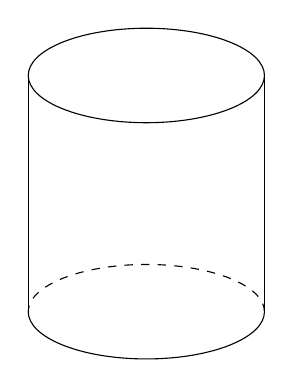
\begin{tikzpicture}
    \newcommand{\size}{1.5}
    \draw (-\size,0) arc (180:360:{\size} and 0.6);
    \draw[dashed] (\size,0) arc (0:180:{\size} and 0.6);
    \draw (-\size,\size+\size) arc (180:360:{\size} and 0.6);
    \draw (\size,\size+\size) arc (0:180:{\size} and 0.6);
    \draw (-\size,0)--(-\size,\size+\size);
    \draw (\size,0)--(\size,\size+\size);
    %\draw[dashed] (\size,0)--(0,0)--(0,\size+\size);
    %\node at (0,-\size+\size/4) {\textit{A right cylinder.}};
    %\filldraw (0,0) circle (1pt);
    %\node at (\size/2,\size/8) {$r$};
    %\node at (\size/6,\size) {$h$};
    \end{tikzpicture}
    \hspace{1.5cm}
    %\textit{A right cylinder.}
    %\\[1\baselineskip]
    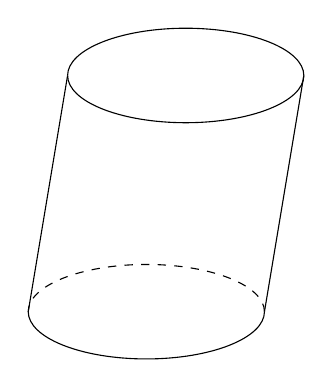
\begin{tikzpicture}
    \newcommand{\size}{1.5}
    \newcommand{\slant}{0.5}
    \draw (-\size,0) arc (180:360:{\size} and 0.6);
    \draw[dashed] (\size,0) arc (0:180:{\size} and 0.6);
    \draw (-\size+\slant,\size+\size) arc (180:360:{\size} and 0.6);
    \draw (\size+\slant,\size+\size) arc (0:180:{\size} and 0.6);
    \draw (-\size,0)--(-\size+\slant,\size+\size);
    \draw (\size,0)--(\size+\slant,\size+\size);
    %\draw[dashed] (\size,0)--(0,0);
    %\draw[dashed] (\size+\slant,0)--(\size+\slant,\size+\size);
    %\node at (0,-\size+\size/4) {\textit{An oblique cylinder.}};
    %\filldraw (0,0) circle (1pt);
    %\node at (\size/2,\size/8) {$r$};
    %\node at (\slant+\size+\size/6,\size/5+\size/5+\size/5+\size/5) {$h$};
    \end{tikzpicture}
\end{center}

As examples, we prove the volume formulas for cylinders/prisms and cones/pyramids, leaving the volume of the sphere as an exercise.

\begin{exam}
The volume of a prism/cylinder with a base of area $B$ and a height of $h$ is $Bh.$
\end{exam}

The proof follows obviously by the definition.

\begin{pro}
Let the reference plane be one of the bases. Then note that the cross-section always has area $B$ over a height of $h.$ Let $k$ be the distance of the cross-section from the base. Then the volume is $\int\limits_{0}^h Bkdk=Bh.$
\end{pro}

If you've ever taken geometry class, you might wonder why the cone and pyramid volume formulae have a coefficient of $\frac{1}{3}.$ Perhaps you have may be suspecting by now that the reason is that $\int x^2dx=\frac{x^3}{3}+C;$ we demonstrate how this produces the coefficient of $\frac{1}{3}.$\footnote{Note that the coefficient of $x^3$ is $\frac{1}{3}$ in the antiderivative.}

\begin{pro}
Let the reference plane be the plane through the apex parallel to the base and let $k$ be the distance of the cross-section from the reference plane. (The cross-section lies on the same side of the reference plane as the base.)

Then by similarity, the volume is $\int\limits_0^k B\frac{k^2}{h^2}dk=\frac{B}{h^2}\int\limits_0^k k^2dk=\frac{B}{h^2}\cdot\frac{h^3}{3}=\frac{Bh}{3}.$
\end{pro}

To finish off, prove the volume of a sphere yourself.

\begin{theo}[Volume of a Sphere]
The volume of a sphere with radius $r$ is $\frac{4\pi r^3}{3}.$
\end{theo}

Surface area is actually surprisingly tricky to define; however, we just need a couple of properties to give an idea of how to work with them.

\begin{fact}[Additivity]
The surface area of an object is the sum of the surface area of its parts.
\end{fact}

\begin{fact}[Surface Area of Flat Shapes]
The surface area of a flat shape is the same as the area of the flat shape.
\end{fact}

\begin{fact}[Straight Lines]
If part of the surface consists of lines, then the surface area of that part can be found by integrating the lengths of the lines.
\end{fact}
As an example, consider the side of a cylinder or the lines joining the apex of a cone to the circumference of its base.

\begin{fact}[Curves]
If part of the surface consists of curves, then the surface area of that part can be found by integrating the lengths of the curves.
\end{fact}

Before we move onto the surface area of a sphere, convince yourself that surface areas can be found through integration as a natural consequence of these properties.

\begin{theo}[Surface Area of a Sphere]
The surface area of a sphere with radius $r$ is $4\pi r^2.$
\end{theo}

\begin{pro} % THIS IS WRONG: FIX PLS
We instead prove that the surface area of a hemisphere, not counting the base, is $2\pi r^2.$

We integrate about the arc of the circumference. Let $\theta$ be the angle a point on the cross-section forms with the radius containing the foot from the point onto the base. Then we integrate about $t=r\theta.$ Note integrating the circumferences gives
\[\int_0^{\frac{\pi r}{2}}2\pi r\cos\frac{t}{r}dt=2\pi r^2.\]
Multiplying by $2$ implies that the surface area of the sphere is $4\pi r^2.$

\begin{center}
    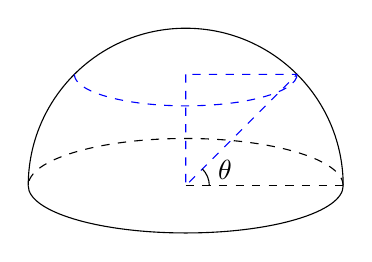
\begin{tikzpicture}
%  \shade[ball color = gray!40, opacity = 0.4] (0,0) circle (2cm);
  \draw (2,0) arc (0:180:2);
  \draw [blue,dashed](-1.41421356,1.41421356) arc (180:360:1.41421356 and 0.4);
  \draw (-2,0) arc (180:360:2 and 0.6);
\draw[dashed] (2,0) arc (0:180:2 and 0.6);
\draw[blue,dashed] (0,1.41421356)--(0,0)--(1.41421356,1.41421356)--cycle;
\draw[dashed] (0,0)--(2,0);
\draw (0.3,0) arc (0:45:0.3);
\node at (0.5,0.2) {$\theta$};
%  \fill[fill=black] (0,0) circle (1pt);
%  \draw[dashed] (0,0 ) -- node[above]{$r$} (2,0);
\end{tikzpicture}
\end{center}
\end{pro}

\begin{exer}
If we try to integrate about the height, as in
\[\int_{0}^r 2\pi\sqrt{r^2-k^2}dk=2\pi\int_{0}^r \sqrt{r^2-k^2}dk,\]
we end up getting that the surface area of a hemisphere is $\frac{\pi r^2}{2}.$ Why is this wrong?
\end{exer}

% https://artofproblemsolving.com/community/q2h2174277p16212703

\subsubsection{Rotating About An Axis: aka. Disks, Washers, and Shells}

For those of you taking or have taken high-school calculus, you will know this as the disk and washer method, as well as the shell method. Despite the specific nomenclature of the disk and washer method, the underlying principles are quite intuitive.

\begin{theo}[Disk Method]
To find the volume of layered disks perpendicular to an axis $\ell$ (these disks will usually be generated through rotation on the coordinate axis), evaluate
\[\int_a^b R(x)dx,\]
where $R(x)$ is the radius of the disk $x$ above an arbitrary base.
\end{theo}

This is (informally) apparent from Cavalieri's principle.\footnote{We do not include the actual proof here, because that is out of the scope of this handout.}

\begin{exam}[Gabriel's Horn]
The graph of $xy=1$ where $x\geq 1$ is rotated about the $x$ axis. Find the volume of the resultant solid, if it is finite at all.
\end{exam}

\begin{sol}
Note that this is an improper integral; we are asked to evaluate
\[\lim\limits_{b\to\infty}\pi\int_1^b \left(\frac{1}{x}\right)^2dx=\lim\limits_{b\to\infty}\pi\left(-\frac{1}{b}-\left(-\frac{1}{1}\right)\right)=\pi.\]
\end{sol}

\begin{exer}[Extension of Gabriel's Horn]
What if our problem with Gabriel's Horn had no domain restrictions; that is, what would the volume have been had we rotated the entirety of $xy=1$ around the $x$ axis? Would it still have been finite?
\end{exer}

The disk method extends pretty naturally to the washer method. The question asked is ``what happens to the volume if I cut circles of varying radiuses out of each layer?'' and the answer is, ``the cutout can also be integrated; evaluate the volume of the part you cut out.''

\begin{theo}[Washer Method]
Say we are finding the volume of the rotation of a curve around a line $\ell.$ We integrate about a plane perpendicular to the axis $\ell;$ if the maximum distance from a point to the axis is $R(x)$ and the minimum distance from a point to the axis is $r(x)$ on the plane $x$ \db{directed} units away from an arbitrary base, then the volume of the curve is
\[\int_a^b (R(x)^2-r(x)^2)dx,\]
provided that \db{every value between the minimum and maximum on each plane is somehow covered by the rotation}.\footnote{In high-school calculus classes, this will usually be the case. High-school calculus contests such as Integration Bee will probably not ask you to know this.}

In terms of the coordinate plane, you want the integral
\[\int_a^b (R(x)^2-r(x)^2)dx,\footnote{I am aware the formula is the same. No, it is not a coincidence or a mistake.}\]
where $y=R(x)$ is the outer radius (larger value) and $y=r(x)$ is the inner radius (smaller value) at $x.$
\end{theo}

\begin{remark}
This can easily be generalized to weirder curves with several ``cutouts;'' however, the computation becomes worse.
\end{remark}

A variant of the dish and washer method is the \db{shell} method. The primary difference is that instead of integrating about the axis of revolution, we integrate instead about a line \db{perpendicular} to the axis of revolution.

\begin{theo}[Shell Method]
Say we are rotating some function $y=f(x)$ with bounds $(a,b)$ around the \db{y}-axis. Then the volume of the resultant solid is
\[2\pi\int_a^b xydx.\footnote{Another way to write the sum is $2\pi\int_a^b xf(x)dx.$}\]
\end{theo}

\begin{pro}
We could probably do this just with pure integral manipulation.\footnote{For anyone interested, the integral manipulation follows:} However, to do this would basically be missing the entire picture; as those of you more familiar with contest math might already have noticed, $2\pi$ strongly suggests the circumference of a circle.

It turns out that $2\pi xy$ actually represents the lateral surface area of a cylinder. I will let the following diagram do the rest of the talking for me.

\begin{center}
\begin{tikzpicture}[scale=0.5]
\draw [color=dennispurple,domain=0:8] plot ({\x}, {-(\x*1/2-1)^2+9});

\draw [color=importantred, pattern = north west lines, pattern color = thmred, bend left=30] (2,0)--(2,9) to (-2,9)--(-2,0) (2,0) to (-2,0);

\draw [color=importantred,bend right=40] (2,9) to (-2,9);

\draw [color=blue] (0,9)--(2,9);

\draw[->] (0,0) -- (10,0);
\draw[->] (0,0) -- (0,11);

\node at (1,9) [anchor = south]{$x$};

\node at (2,4.5) [anchor=west]{$y$};
\end{tikzpicture}
\end{center}

Since the sum of these lateral surface areas is equivalent to the volume, we are done.
\end{pro}

We present a somewhat funny solution to Gabriel's Horn with this.

\begin{sol}[(Gabriel's Horn)]
Note that by symmetry, this is equivalent to rotating $y\geq 1$ around the $y$ axis, or $0\leq x\leq 1$ around the $y$ axis. Shift the function down by $1,$ since the range $0\leq y\leq 1$ is not going to be rotated around the axis. Now by the Shell Method, this is just
\[2\pi\int_0^1 x\left(\frac{1}{x}-1\right)dx=\pi.\]
Hilarious.
\end{sol}

So what would we do if we encountered an axis of integration that was not an axis? All we have to do is transform it.

\begin{exam}
Consider the curve bound by $y=-x^2+4$ and $y=0.$ Find the volume of the curve when rotated around $x=-1.$
\end{exam}

\begin{sol}
We shift the axis of rotation to $x=0$, attaining $y=-(x-1)^2+4$ as the new equation of our curve. Clearly, $|\sqrt{y}+1|>|\sqrt{y}-1|$ for positive $y,$ so we can actually disregard the second quarant altogether.

Now we just use the Shell Method; the answer is
\[2\pi\int_0^3 x(-(x-1)^2+4)dx=\frac{45}{2}.\]
\end{sol}

To finish off this section, we end with a quite insane example.

\begin{exam}
The curve $xy=1,$ defined for $1\leq x\leq a$ for positive $a>1,$ is rotated around the line $y=x.$ Find, in terms of $a,$ the volume of the resultant solid.
\end{exam}

\begin{sol}
Read the appendix for an explanation of the techniques used here.

Rotate the axes by $45^{\circ}$ and note that $x=x'\cos 45^{\circ}-y'\sin 45^{\circ}$ and $y=x'\sin 45^{\circ}+y\cos 45^{\circ},$ where $x'$ and $y'$ are the new coordinates. Then
\[\frac{1}{2}(x'-y')(x'+y')=1,\]
or
\[x'^2-y'^2=2,\]
where the domain is $x'\geq \sqrt{2}$ and the range is $y'\leq 0.$ Now we need to interpret $x\leq a;$ note that $x'=x\cos 45^{\circ}+y\sin 45^{\circ}=\frac{x+y}{\sqrt{2}}.$ By AM-GM, the larger $x$ is (or the further $x$ is from $y$), the larger $x+y$ becomes. Thus, $x'\leq \frac{a+\frac{1}{a}}{\sqrt{2}}=\frac{a^2+1}{a\sqrt{2}}.$

Now we can just use the washer method; the integral is
\[\pi\int_{\sqrt{2}}^{\frac{a^2+1}{a\sqrt{2}}}(-\sqrt{x^2-2})^2dx=\pi\int_{\sqrt{2}}^{\frac{a^2+1}{a\sqrt{2}}}(x^2-2)dx=\pi\Eval{\left(\frac{x^3}{3}-2x\right)}{\sqrt{2}}{\frac{a^2+1}{a\sqrt{2}}}=\frac{(a-1)^4(a^2+4a+1)}{6\sqrt{2}a^3}\pi.\]
\end{sol}

\subsection{Polar Functions}

To determine a point in $\mathbb{R}^2,$ you need two pieces of information. However, these two pieces of information need not directly be the $x$ and $y$ coordinates (rectangular form). They can be in another form: polar.

In polar coordinates, a point is defined with a distance from the origin and an angle.

\begin{defi}[Polar Coordinates]
The point $(r,\theta)$ in polar coordinates is the point $(r,0)$ (rectangular coordinates) rotated by $\theta$ counterclockwise around the origin. In other words, it is equivalent to $(r\cos\theta, r\sin\theta)$ in rectangular coordinates.
\end{defi}

Curves can be defined in the $xy$ plane, like $x^2+y^2=1.$ However, we can also define the radius as a function of $\theta.$ Consider $r=1$ as a very simple example: this is a circle because the output is the same for all $\theta.$ Another example is $r=\cos\theta;$ this turns out to be the following graph.
\begin{center}
\begin{tikzpicture}[scale=1.2]
\draw[->] (-0.5,0)--(1.5,0);
\draw[->] (0,-1)--(0,1);
\draw (0.5, 0) circle (0.5);

\end{tikzpicture}
\end{center}

There are plenty of good resources for learning polar coordinates out there, but this handout is not meant to act as an introduction to them. If you don't understand them, I would skip this section entirely.

Let's get to the area of a polar curve.

\begin{theo}[Area of a Polar Curve]
The area of the polar curve
\[r=f(\theta)\]
on the interval $(\alpha,\beta)$ is
\[\int_{\alpha}^{\beta}\frac{1}{2}\theta r^2d\theta.\]
\end{theo}

The proof is fundamentally identical to the \hyperref[theo:fun]{rectangular version}, even if it looks different.

\begin{pro}
Say $F(\theta)=\int_{\alpha}^{\theta}\frac{1}{2}\gamma r^2d\gamma.$ (We use $\gamma$ just because we're using $\theta$ as the input of the function; it is identical to the rest of the integrals.)

Note that
\[F'(\theta)=\lim\limits_{\epsilon\to 0}\frac{F(\theta+\epsilon)-F(\theta)}{\epsilon}=\lim\limits_{\epsilon\to 0}\frac{\int_{\theta}^{\theta+\epsilon}f(\gamma)d\gamma}{\epsilon}=\frac{\frac{\epsilon}{2\pi}\cdot \pi f(\theta)^2}{\epsilon}=\frac{f(\theta)^2}{2}.\]

Note that if $F'(\theta)=f(\theta),$ then by the Fundamental Theorem of Calculus,
\[F(\beta)-F(\alpha)=\int_{\alpha}^{\beta} \theta r^2d\theta.\]

\begin{center}
\begin{tikzpicture}[scale=1.5]
\draw[thick,->,>=latex] (-1,0)--(3,0) node[above] {$x$};
\draw[thick,->,>=latex] (0,-2)--(0,2) node[left] {$y$};
\draw[domain=0:360, samples=500] plot (\x:{1+cos(\x)});
\filldraw[pattern = north west lines, pattern color = importantred, draw=darkblue, dashed] (0,0) -- (1.95465406,0.344658249) arc (10:20:1.98480775) -- cycle;
\end{tikzpicture}
\end{center}
\end{pro}

Here are some motivating remarks. This is all based on the same idea as Riemann Sums for rectangles: where we added rectangles before, we are adding circular arcs now. If you wanted to be a little less rigorous, you could say that you're ``adding'' a lot of small circular arcs together and skip the Fundamental Theorem of Calculus stuff altogether. \footnote{That isn't to say this proof is rigorous at all, because we haven't been taking things from an analysis perspective whatsoever.}

Why is $r^2$ squared? Think in terms of dimensional analysis: if the radius is doubled, it would quadruple the area, which is why we need the square. And why is there a factor of $\frac{1}{2}?$ Because with a circular arc of radius $r$ and angle $\epsilon,$ the area is $\frac{\epsilon}{2\pi}(\pi r^2)=\frac{1}{2}r^2.$

% discuss riemann curves

% https://math.libretexts.org/Bookshelves/Calculus/Map%3A_Calculus__Early_Transcendentals_(Stewart)/10%3A_Parametric_Equations_And_Polar_Coordinates/10.04%3A_Areas_and_Lengths_in_Polar_Coordinates

\subsection{Length of a Curve}

There are three ways to describe a curve: through rectangular, parametric, and polar coordinates.\footnote{Strictly speaking, polar curves are a subset of parametric curves.} Each of them has their own length formula. It's easy to memorize them, but the important thing is understanding how they are all the same.

We begin with parametric curves and show that the other two are equivalent.

\begin{theo}[Arc Length with Parametric Curves]
The arc length of a parametric function from $a$ to $b$ is
\[\int_a^b \sqrt{\left(\frac{dx}{dt}\right)^2+\left(\frac{dy}{dt}\right)^2}dt.\]
\end{theo}

Here is a short explanation of why this \textit{should} be true. Let me emphasize that \db{this is not a proof}.

Note that the distance between $(x(t),y(t))$ and $(x(t+\epsilon),y(t+\epsilon))$ for small $\epsilon$ is
\[\sqrt{(dx)^2+(dy)^2}\]
by the Pythagorean Theorem, and note this is equal to
\[\sqrt{\left(\frac{dx}{dt}\right)^2+\left(\frac{dy}{dt}\right)^2}dt\]
as desired.

\begin{center}
\begin{tikzpicture}
\draw[->] (-4,0)--(3,0);
\draw[->] (0,-2)--(0,4);
\draw[domain=-4:3, samples=500] plot(\x,{\x^3*1/10+\x*\x*2/5-\x*4/5-4/5});
\draw (2.2,0.441)--(2.6,0.441);
\node at (2.4,0.441) [below] {$dx$};
\draw (2.6,0.441)--(2.6,1.582);
\node at (2.6,1.0115) [right] {$dy$};
\end{tikzpicture}
\end{center}

\begin{theo}[Arc Length in Rectangular Form]
The arc length of a rectangular function from $a$ to $b$ is
\[\int_a^b \sqrt{1+\left(\frac{dy}{dx}\right)^2}dx.\]
\end{theo}

Notice that this just follows from the parametric curve
\begin{align*}
x&=t \\
y&=f(t).
\end{align*}

\begin{theo}[Arc Length in Polar Form]
The arc length of a polar function $r=f(\theta)$ from $\alpha$ to $\beta$ is
\[\int_{\alpha}^{\beta}\sqrt{r^2+\left(\frac{dr}{d\theta}\right)^2}d\theta.\]
\end{theo}

\begin{proof}
This is just a standard parametric substitution plus some differentiation.

Note $x=f(\theta)\cos\theta$ and $y=f(\theta)\sin\theta,$ so by the Product Rule,
\[\frac{dx}{d\theta}=f'(\theta)\cos\theta-f(\theta)\sin\theta=\frac{dr}{d\theta}\cos\theta-r\sin\theta,\]
and similarly,
\[\frac{dy}{d\theta}=\frac{dr}{d\theta}\sin\theta+r\cos\theta.\]
Now note
\begin{align*}
\sqrt{\left(\frac{dx}{d\theta}\right)^2+\left(\frac{dy}{d\theta}\right)^2}&=\sqrt{\left(\frac{dr}{d\theta}\cos\theta-r\sin\theta\right)^2+\left(\frac{dr}{d\theta}\sin\theta+r\cos\theta\right)^2} \\
&=\sqrt{\left(\frac{dr}{d\theta}\right)^2(cos^2\theta+\sin^2\theta)+r\frac{dr}{d\theta}(-2\sin\theta\cos\theta+2\sin\theta\cos\theta)+r^2(\sin^2\theta+\cos^2\theta)} \\
&=\sqrt{r^2+\left(\frac{dr}{d\theta}\right)^2}.
\end{align*}
So the initial parametric integral simplifies to
\[\int_{\alpha}^{\beta}\sqrt{r^2+\left(\frac{dr}{d\theta}\right)^2}d\theta.\]
\end{proof}

% http://www.mathwords.com/a/arc_length_of_a_curve.htm

\subsection{Bound Tricks}
It is often hard to bound an integral. Here are a few tricks:
\begin{itemize}
    \item If $1+a^x$ is in the denominator with bounds $-b$ to $b$, then apply $u=-x$.
    \item If the integrand is in the form $\frac{f(x-c)}{f(x-c)+f(-x+d)}$ with bounds from $a$ to $b$, and $a+b=c+d,$ then apply $u=a+b-x$. This is usually seen in the form $u=\frac{pi}{2}-x$ for trigonometric functions over $\paren{0,\frac{\pi}{2}}$ or $u=1-x$ over $(0,1)$.
    \item If $x^2+a^2$ is in the denominator with bounds 0 to $\infty$ or 1 to $a$ (which is common with $\ln x$ and $\arctan x$), apply $u=\frac{a}{x}$.
\end{itemize}

\begin{exer}
Evaluate $\int_{-\infty}^{\infty} \frac{1}{(1+x^2)(1+e^x)}\,dx$.
\end{exer}

\subsection{Weierstrass Substitution}
The \db{Weierstrass substitution} is simply $t=\tan\paren{\frac{x}{2}}$. Under this substitution, we have
$$\sin x=\frac{2t}{1+t^2} \qquad \cos x=\frac{1-t^2}{1+t^2} \qquad dx=\frac{2}{1+t^2}\,dx.$$
his allows us to turn trigonometric expressions into rational functions. Using $t=\tanh\paren{\frac{x}{2}}$, we can similarly derive
$$\sinh x=\frac{2t}{1-t^2} \qquad \cosh(x)=\frac{1+t^2}{1-t^2} \qquad dx=\frac{2}{1-t^2}\,dx.$$

\begin{exer}
Evaluate $\int_0^{\frac{\pi}{2}} \frac{1}{3+\cos x}\,dx$.
\end{exer}

\section{List of Integration Techniques}
Your toolbox, with a few additions not covered in this handout.
\begin{itemize}
    \item Substitutions
    \begin{itemize}
        \item $u$-Substitution
        \item Trigonometric Substitution
        \item Weierstrass Substitution
        \item Bounding Tricks
        \item Inversion (Reverse $u$-Substitution)
    \end{itemize}
    \item Partial Fraction Decomposition
    \item Integration by Parts
    \begin{itemize}
        \item $u=e^x$
        \item $u'=1$ (i.e. $u=x$)
        \item Tabular Integration (i.e. making a chart)
    \end{itemize}
    \item Parametrization
    \item Feynman's Technique (Differentiation Under the Integral)
\end{itemize}

\problems

\minpt{32}

\psetquote{Oh, I \textit{will} find it. You may pretend he is not here, but I will find him, though I dig forever!}{The Count of Monte Cristo}

\prob{2}{SMT 2018/4}{Compute
\[\int_0^4\frac{dx}{\sqrt{|x-2}}.\]}

\prob{2}{Putnam Calculus Problems 2016-I/1}{Show that for all $x>1,$
\[\int_{1}^x e^{-t^2}dt<\frac{1}{2e}.\]}

\req{2}{}{Find $\int f(x)f'(x)dx.$}

\req{3}{}{Find $\int e^x\sin xdx.$}

\prob{3}{SMT 2018/3}{Find the value of $a$ such that
\[\int_1^a\left(3x^2-6x+3\right)dx=27.\]}

\prob{3}{Vishal Muthuvel}{Find the average value of the function $f(x)=\cos(2x)-\sin(\frac{x}{2})$ on the interval $[\frac{-\pi}{2},\pi]$.}

\prob{4}{}{Evaluate
\[\int \frac{1}{x^2+c}dx.\]}

\prob{4}{SMT 2019/3}{Compute $\int_0^{\pi/4}\cos x-2\sin x\sin 2x dx.$}

\req{4}{AMC 12A 2016/23}{Three numbers in the interval $[0,1]$ are chosen independently and at random. What is the probability that the chosen numbers are the side lengths of a triangle with positive area?}

\prob{6}{MIT OCW}{Evaluate the following limits:
	\[\lim_{n \to \infty} \sum_{i = 1}^n\left[\sqrt{1+\frac{2i}{n}}\right]\frac{2}{n}\]
	\[\lim_{h \to \infty} \frac{1}{h}\int_{2}^{2+h}\sin(x^2)dx.\]
}

\prob{6}{Joe Foster}{Find
\[\int \frac{1}{\sqrt{8x-x^2}}dx.\]}

\prob{6}{SMT Calculus 2019/10}{Evaluate $\int_0^2\frac{\ln(1+x)}{x^2-x+1}\,dx$.}

\prob{6}{David Altizio}{Evaluate \[\int \frac{2x}{x^4 + 1},dx.\]}

\prob{9}{}{Evaluate \[\int \frac{dx}{e^x - 1}.\]}

\req{9}{AMC 10A 2015/25}{Let $S$ be a square of side length $1$.  Two points are chosen independently at random on the sides of $S$.  The probability that the straight-line distance between the points is at least $\tfrac12$ is $\tfrac{a-b\pi}c$, where $a$, $b$, and $c$ are positive integers and $\gcd(a,b,c)=1$.  What is $a+b+c$?}

\prob{9}{SMT 2019/7}{Turn the graph of $y=\frac{1}{x}$ by $45^{\circ}$ counter-clockwise and consider the bowl-like top part of the curve (the part above $y=0$). We let a 2D fluid accummulate in this 2D bowl until the maximum depth of the fluid is $\frac{2\sqrt{2}}{3}.$ What’s the area of the fluid used?\footnote{Reading Section B of the Appendix may help, but is strictly unnecessary.}}

\prob{9}{MIT Integration Bee 2006}{Evaluate $\int_0^{\frac{\pi}{2}}\frac{\cos(x)+\sin(x)}{9+16\sin(2x)}\,dx$.} % u = cos x - sin x i think

\prob{13}{AIME I 2015/15}{A block of wood has the shape of a right circular cylinder with radius $6$ and height $8$, and its entire surface has been painted blue. Points $A$ and $B$ are chosen on the edge of one of the circular faces of the cylinder so that $\overarc{AB}$ on that face measures $120^\text{o}$. The block is then sliced in half along the plane that passes through point $A$, point $B$, and the center of the cylinder, revealing a flat, unpainted face on each half. The area of one of these unpainted faces is $a\cdot\pi + b\sqrt{c}$, where $a$, $b$, and $c$ are integers and $c$ is not divisible by the square of any prime. Find $a+b+c$.
\begin{center}
    \begin{asy}
        import geometry; import olympiad; import cse5; import three; import solids; size(8cm); currentprojection=orthographic(-1,-5,3);  picture lpic, rpic;  size(lpic,5cm); draw(lpic,surface(revolution((0,0,0),(-3,3*sqrt(3),0)..(0,6,4)..(3,3*sqrt(3),8),Z,0,120)),gray(0.7),nolight); draw(lpic,surface(revolution((0,0,0),(-3*sqrt(3),-3,8)..(-6,0,4)..(-3*sqrt(3),3,0),Z,0,90)),gray(0.7),nolight); draw(lpic,surface((3,3*sqrt(3),8)..(-6,0,8)..(3,-3*sqrt(3),8)--cycle),gray(0.7),nolight); draw(lpic,(3,-3*sqrt(3),8)..(-6,0,8)..(3,3*sqrt(3),8)); draw(lpic,(-3,3*sqrt(3),0)--(-3,-3*sqrt(3),0),dashed); draw(lpic,(3,3*sqrt(3),8)..(0,6,4)..(-3,3*sqrt(3),0)--(-3,3*sqrt(3),0)..(-3*sqrt(3),3,0)..(-6,0,0),dashed); draw(lpic,(3,3*sqrt(3),8)--(3,-3*sqrt(3),8)..(0,-6,4)..(-3,-3*sqrt(3),0)--(-3,-3*sqrt(3),0)..(-3*sqrt(3),-3,0)..(-6,0,0)); draw(lpic,(6*cos(atan(-1/5)+3.14159),6*sin(atan(-1/5)+3.14159),0)--(6*cos(atan(-1/5)+3.14159),6*sin(atan(-1/5)+3.14159),8));  size(rpic,5cm); draw(rpic,surface(revolution((0,0,0),(3,3*sqrt(3),8)..(0,6,4)..(-3,3*sqrt(3),0),Z,230,360)),gray(0.7),nolight); draw(rpic,surface((-3,3*sqrt(3),0)..(6,0,0)..(-3,-3*sqrt(3),0)--cycle),gray(0.7),nolight); draw(rpic,surface((-3,3*sqrt(3),0)..(0,6,4)..(3,3*sqrt(3),8)--(3,3*sqrt(3),8)--(3,-3*sqrt(3),8)--(3,-3*sqrt(3),8)..(0,-6,4)..(-3,-3*sqrt(3),0)--cycle),white,nolight); draw(rpic,(-3,-3*sqrt(3),0)..(-6*cos(atan(-1/5)+3.14159),-6*sin(atan(-1/5)+3.14159),0)..(6,0,0)); draw(rpic,(-6*cos(atan(-1/5)+3.14159),-6*sin(atan(-1/5)+3.14159),0)..(6,0,0)..(-3,3*sqrt(3),0),dashed); draw(rpic,(3,3*sqrt(3),8)--(3,-3*sqrt(3),8)); draw(rpic,(-3,3*sqrt(3),0)..(0,6,4)..(3,3*sqrt(3),8)--(3,3*sqrt(3),8)..(3*sqrt(3),3,8)..(6,0,8)); draw(rpic,(-3,3*sqrt(3),0)--(-3,-3*sqrt(3),0)..(0,-6,4)..(3,-3*sqrt(3),8)--(3,-3*sqrt(3),8)..(3*sqrt(3),-3,8)..(6,0,8)); draw(rpic,(-6*cos(atan(-1/5)+3.14159),-6*sin(atan(-1/5)+3.14159),0)--(-6*cos(atan(-1/5)+3.14159),-6*sin(atan(-1/5)+3.14159),8));  add(lpic.fit(),(0,0)); add(rpic.fit(),(1,0));
        // label(rpic,"$A$",(-3,3*sqrt(3),0),W); label(rpic,"$B$",(-3,-3*sqrt(3),0),W); // these didn't work idk
    \end{asy}
\end{center}
}

\pagebreak

\appendix

% \noindent{\LARGE\merri \bfseries Appendix} % you don't even need this tbh

\section{Partial Fraction Decomposition}

The contents of this section can be found on the appendix of \href{https://www.geometryexplorer.xyz/pdfs/AQU-TelescopingNew.pdf}{AQU-Telescoping}, but they are also reproduced here for your convenience.

\begin{defi}[Partial Fraction Decomposition]
The partial fraction decomposition of a fraction
\[\frac{f(x)}{(x-r_1)^{c_1}(x-r_2)^{c_2}\cdots (x-r_n)^{c_n}}\]
is of the form
\[\sum_{i=1}\frac{f_i(x)}{(x-r_i)^{c_i}}=\frac{f_1(x)}{(x-r_1)^{c_1}}+\frac{f_2(x)}{(x-r_2)^{c_2}}+\cdots+\frac{f_n(x)}{(x-r_n)^{c_n}}.\]
\end{defi}

The traditional way to solve this is by setting a system of equations. We take the well-known $\frac{1}{x}-\frac{1}{x+1}$ partial fraction decomposition as an example.

\begin{exam}
Find the partial fraction decomposition of $\frac{1}{x(x+1)}.$
\end{exam}

\begin{sol}
Note that the partial fraction decomposition is of the form
\[\frac{1}{x(x+1)}=\frac{A}{x}+\frac{B}{x+1}.\footnote{We can use $A$ and $B$ as constants because the degree of $x$ and $x+1$ is one less than the degree of $x(x+1).$}\]
Now we multiply out the fraction to get
\[1=A(x+1)+Bx.\]
This implies that $A+B=0$ and that $A=1.$ Thus $B=-1,$ and the PFD is
\[\frac{1}{x}-\frac{1}{x+1}.\]
\end{sol}

We proceed with a harder example.

\begin{exam}[Three Terms]
Find the partial fraction decomposition of $\frac{1}{n(n+1)(n+2)}.$
\end{exam}
\begin{sol}
Let the decomposition be $\frac{1}{n(n+1)(n+2)}=\frac{I}{n}+\frac{J}{n+1}+\frac{K}{n+2}.$ This implies that \[I(n+1)(n+2)+J(n)(n+2)+K(n)(n+1)=1.\]
We see that the following system of equations results from coefficient matching: $$n^2(I+J+K)=0\implies I+J+K=0$$ $$n(3I+2J+K)=0\implies 3I+2J+K=0$$ $$2I=1.$$ Solving gives us $I=1/2, J=-1, K=1/2,$ which means our partial fraction decomposition is $\frac{1/2}{n}-\frac{1}{n+1}+\frac{1/2}{n+2}.$
\end{sol}

In calculus classes, the forbidden values method is taught, though usually with little explanation given as to why it should be true or why it should work. My goal is to give the reader a feeling for why this should be true, give concrete examples as to when it works, and show when it doesn't.

\begin{theo}[Forbidden Values]
Given some partial fraction decomposition
\[\frac{f(x)}{g_1(x)g_2(x)\cdots g_n(x)}=\frac{f_1(x)}{g_1(x)}+\frac{f_2(x)}{g_2(x)}+\cdots+\frac{f_n(x)}{g_n(x)},\]
the functions $f_1,f_2,\ldots, f_n$ can be determined via substituting the roots of $g_i(x)$ for all $1\leq i\leq n$ into
\[f(x)=f_1(x)g_2(x)\cdots g_n(x)+\cdots+f_n(x)g_1(x)\cdots g_{n-1}(x).\]
\end{theo}

The natural instinct to have after using this `trick' a couple times is, ``Wait, why does this actually work?'' and it is very easy to just relegate this to a trick that you don't think about. However, there is a well-founded reason that this works, and it is rooted in polynomial and root analysis. We remind the reader of the following theorem from \db{AQU-Factorize}.

\begin{theo}[Infinite Roots]
If a degree $n$ polynomial has more than $n$ roots, it must have infinite roots.
\end{theo}

Now the proof follows naturally.

\begin{pro}[of Forbidden Values]
Note that as
\[\frac{f(x)}{g_1(x)g_2(x)\cdots g_n(x)}=\frac{f_1(x)}{g_1(x)}+\frac{f_2(x)}{g_2(x)}+\cdots+\frac{f_n(x)}{g_n(x)}\]
has infinite roots, so must 
\[f(x)=f_1(x)g_2(x)\cdots g_n(x)+\cdots+f_n(x)g_1(x)\cdots g_{n-1}(x).\]
This implies that
\[f(x)-(f_1(x)g_2(x)\cdots g_n(x)+\cdots+f_n(x)g_1(x)\cdots g_{n-1}(x))=0\]
for all values of $x,$ even the roots of $g_i(x).$
\end{pro}

Forbidden values can instantly tell us how a fraction decomposes. We present the following corollary that eliminates most algebraic manipulation from PFD, aside from the initial factorization of the denominator.

\begin{theo}[Only Linear $g_i$ Work]
Given some partial fraction decomposition
\[\frac{f(x)}{g_1(x)g_2(x)\cdots g_n(x)}=\frac{f_1(x)}{g_1(x)}+\frac{f_2(x)}{g_2(x)}+\cdots+\frac{f_n(x)}{g_n(x)},\] where $g_i$ is of the form $(x-r_i)^{c_i},$
\[f_i(r_i)=\frac{f(r_i)}{\prod\limits_{1\leq k\leq n, k\neq i}g_i(r_i)},\] where $r_i$ is the root of $g_i.$

In the case where all $g_i$ are linear, $f_i$ are all constant, so \[f_i=\frac{f(r_i)}{\prod\limits_{1\leq k\leq n,k\neq i}g_i(r_i)}.\]
\end{theo}

Keep in mind that this only explicitly describes the values achieved from forbidden values; you should almost always clear the fractions and substitute the forbidden values yourself instead of trying to recall the exact formula. The corollary does little good especially when some $g_i$ is not linear. If no $g_i$ are linear, the forbidden values method is completely useless, since no $f_i$ will be linear. In fact, forbidden values works exactly when $g_i$ is linear, even if other $g$ are not.

Let me state it more explicitly: \db{substituting forbidden values only works for linear $g_i$}.

\begin{exam}
Find the partial fraction decomposition of $\frac{1}{x(x+1)}.$
\end{exam}

\begin{sol}
With our new forbidden values method in hand, we set
\[\frac{1}{x(x+1)}=\frac{f_1}{x}+\frac{f_2}{x+1}\]
and multiply out to get
\[1=f_1\cdot (x+1)+f_2\cdot (x).\]
Since $x$ and $x+1$ are both linear, $f_1$ and $f_2$ are both constants. Substituting $x=0$ gives $f_1=1$ and $x=-1$ gives $f_2=-1,$ so our PFD is
\[\frac{1}{x(x+1)}=\frac{1}{x}-\frac{1}{x+1}.\]
\end{sol}

Here's a partial forbidden values solution of a PFD; one of the terms in the denominator is linear while the other is not.

\begin{exam}
Find the partial fraction decomposition of $\frac{2x^2-4x+1}{(x-1)^2(x-2)}.$
\end{exam}

\begin{sol}
Note that the fraction decomposes into the form
\[\frac{2x^2-4x+1}{(x-1)^2(x-2)}=\frac{f_1(x)}{(x-1)^2}+\frac{f_2(x)}{x-2},\]
which is equivalent to
\[2x^2-4x+1=f_1(x)(x-2)+f_2(x)(x-1)^2.\]
Plugging in $x=1$ yields $-1=-f_1(1)$ or $1=f_1(1),$ and $x=2$ yields $1=f_2(2).$ Degree analysis only tells us that $f_2$ is constant, or $f_2(x)=1.$ Now we have
\[2x^2-4x+1=f_1(x)(x-2)+(x-1)^2.\]
Now we directly solve for $f_1.$ Note that the equation is equivalent to
\[x^2-2x=f_1(x)(x-2)\]
\[f_1(x)=x.\]
Thus, the PFD is
\[\frac{2x^2-4x+1}{(x-1)^2(x-2)}=\frac{x}{(x-1)^2}+\frac{1}{x-2}.\]
\end{sol}

Here is a crown example of the forbidden values method.

\begin{exam}[AMC 10A 2019/24]
Let $p$, $q$, and $r$ be the distinct roots of the polynomial $x^3 - 22x^2 + 80x - 67$. It is given that there exist real numbers $A$, $B$, and $C$ such that\[\dfrac{1}{s^3 - 22s^2 + 80s - 67} = \dfrac{A}{s-p} + \dfrac{B}{s-q} + \frac{C}{s-r}\]for all $s\not\in\{p,q,r\}$. What is $\tfrac1A+\tfrac1B+\tfrac1C$?
\end{exam}

\begin{sol}
This is the same as solving for $A,B,C$ such that
\[1=A(s-q)(s-r)+B(s-r)(s-p)+C(s-p)(s-q).\]
Substitute the forbidden values of $s=p,q,r$ to get
\begin{align*}
1&=A(p-q)(p-r) \\
1&=B(q-r)(q-p) \\
1&=C(r-p)(r-q),
\end{align*}
which we get from substituting $s=p,q,r,$ respectively. This then implies
\begin{align*}
\frac{1}{A}&=(p-q)(q-r) \\
\frac{1}{B}&=(q-r)(q-p) \\
\frac{1}{C}&=(r-p)(r-q).
\end{align*}
At this point we can just finish with Vieta's Formulas. Note that
\[\frac{1}{A}+\frac{1}{B}+\frac{1}{C}=(p-q)(p-r)+(q-r)(q-p)+(r-p)(r-q)=\]
\[p^2-pq-pr+qr+q^2-qr-qp+rp+r^2-rp-rq+pq=\]
\[(p+q+r)^2-3(pq+qr+rp)=22^2-3\cdot 80=244.\]
\end{sol}

\begin{exer}[Adapted from AoPS Calculus 5.35]
Find the partial fraction decomposition of
\[\frac{3}{x^3-1}.\]
\end{exer}

\section{Rotation of Coordinates}

This is just for fun for anyone who really wants to understand the last example presented.

\begin{theo}[Rotation of Axes]
If the coordinate axes $x,y$ are rotated by $\theta$ to produce a new coordinate system $x',y',$ then a point $(x,y)$ in the old coordinate system becomes $(x',y')=(x\cos\theta + y\sin\theta,-x\sin\theta + y\cos\theta).$
\begin{center}
\begin{tikzpicture}[scale=3]
\coordinate (a) at (1,0);
\coordinate (b) at (0,0);
\coordinate (c) at (0.866,0.5);

\coordinate (p) at (1/3,2/3);

\draw[line width = 0.2mm, dashed, darkblue] (0,2/3)--(p)--(1/3,0);
\draw[line width = 0.2mm, dashed, importantred] ($(b)!(p)!(c)$)--(p)--($(-0.5,0.866)!(p)!(b)$);

\draw pic["$\theta$", draw, angle eccentricity=1.5, angle radius=0.6cm]
    {angle=a--b--c};


\draw[line width = 0.2mm, darkblue] (1,0)--(0,0)--(0,1);
\draw[line width = 0.2mm, importantred] (-0.5,0.866)--(0,0)--(0.866,0.5);
\end{tikzpicture}
\end{center}
\end{theo}

Understanding this theorem requires a good bit of experience with polar coordinates. We express the coordinates of the point in polar form; if $(x,y)=(r,\alpha),$ then by definition, $(x',y')=(r,\alpha-\theta).$ Now by the sine and cosine addition formulae,
\[x'=r\cos(\alpha-\theta)=r\cos\alpha\cos\theta+r\sin\alpha\sin\theta=x\cos\theta+y\sin\theta\]
\[y'=r\sin(\alpha-\theta)=r\sin\alpha\cos\theta-r\cos\alpha\sin\theta=y\cos\theta-x\sin\theta.\]

That's all fine and dandy, but this is the perfect excuse to show you a little bit of linear algebra. Note that the above system of equations can perfectly be expressed in the following equation:
\[\begin{bmatrix}x' \\ y'\end{bmatrix}=\begin{bmatrix}\cos (-\theta) & -\sin(-\theta) \\ \sin(-\theta) & \cos(-\theta)\end{bmatrix}\begin{bmatrix}x \\ y\end{bmatrix}.\]
Why do we express the rotation matrix like this? Because what we're doing is really equivalent to \db{rotating the point} by $-\theta$ around the origin. Thus, commonly, the rotation matrix is defined as following.

\begin{defi}[Rotation Matrix]
The two-dimensional rotation matrix $R=\begin{bmatrix}\cos\theta & -\sin\theta \\ \sin\theta & \cos\theta\end{bmatrix}$ is used to rotate some two-dimensional vector $\vec{v}$ by $\theta,$ and the rotation is done by
\[R\vec{v}=\vec{v_1},\]
where $\vec{v_1}$ is the resultant vector.
\end{defi}

Keep in mind this definition follows from the use of polar coordinates and the sine and cosine addition formulae. With the rotation matrix, we can easily write the converse of our original transformation:
\[\begin{bmatrix}x \\ y\end{bmatrix}=\begin{bmatrix}\cos \theta & -\sin\theta \\ \sin\theta & \cos-\theta\end{bmatrix}\begin{bmatrix}x' \\ y'\end{bmatrix}.\]

\begin{exam}
Evaluate
\[\begin{bmatrix}\sqrt{6}+\sqrt{2} & -\sqrt{6}+\sqrt{2} \\ \sqrt{6}-\sqrt{2} & \sqrt{6}+\sqrt{2}\end{bmatrix}^6.\]
\end{exam}

\begin{sol}
The first instinct of someone who sees this problem might be to diagonalize; however, the expressions $\sqrt{6}\pm\sqrt{2}$ remind of us $\cos 15^{\circ}$ and $\sin 15^{\circ}.$ Indeed, note that if our matrix is $A,$
\[A=4R_{15^{\circ}},\]
where $R_{\theta}$ is defined as the rotation matrix of $\theta.$ Thus,
\[A^6=4^6R_{15^{\circ}}^6,\]
and \[R_{15^{\circ}}^6=R_{90^{\circ}}\footnote{This is because six rotations of $15^{\circ}$ are equivalent to a rotation of $90^{\circ}.$}=\begin{bmatrix}0 & -1 \\ 1 & 0\end{bmatrix},\]
so the answer is
\[\begin{bmatrix}0 & -4^6 \\ 4^6 & 0\end{bmatrix}.\]
\end{sol}

Now we condense the exposition above into a proof of our initial theorem.

\begin{pro}
This is equivalent to rotating the point by $-\theta$ around the origin; thus, we multiply
\[\begin{bmatrix}\cos (-\theta) & -\sin(-\theta) \\ \sin(-\theta) & \cos(-\theta)\end{bmatrix}\begin{bmatrix}x \\ y\end{bmatrix}=\begin{bmatrix}\cos \theta & \sin\theta \\ -\sin\theta & \cos\theta\end{bmatrix}\begin{bmatrix}x \\ y\end{bmatrix}=\begin{bmatrix}x\cos \theta + y\sin \theta \\ -x \sin \theta + y\cos \theta\end{bmatrix}.\]
\end{pro}

I cannot stress this enough: \db{matrices are convenient representations of linear mappings}, not random arrays of numbers; hopefully this has shown you one of the fantastic uses of matrices and you don't write them off as ``arcane magic we learned about in high school that one time.'' There's a reason I included the last example in Rotating About An Axis, and it wasn't just to show how transformations could make Disks, Washers, and Shells usable.

\end{document}